\documentclass[11pt, oneside]{article}   	% use "amsart" instead of "article" for AMSLaTeX format
\usepackage{geometry}                		% See geometry.pdf to learn the layout options. There are lots.
\geometry{letterpaper}                   		% ... or a4paper or a5paper or ... 
%\geometry{landscape}                		% Activate for rotated page geometry
%\usepackage[parfill]{parskip}    		% Activate to begin paragraphs with an empty line rather than an indent
\usepackage{graphicx}				% Use pdf, png, jpg, or eps§ with pdflatex; use eps in DVI mode
								% TeX will automatically convert eps --> pdf in pdflatex		
\usepackage{amssymb}


\addtolength{\oddsidemargin}{-.875in}
	\addtolength{\evensidemargin}{-.875in}
	\addtolength{\textwidth}{1.75in}

	\addtolength{\topmargin}{-.875in}
	\addtolength{\textheight}{1.75in}

%SetFonts

%SetFonts


\title{Analysis of M838 data for 2022 ARVO Abstract}
\author{Nicolas P. Cottaris}
\date{}							% Activate to display a given date or no date

\begin{document}
\maketitle
\section{Methods}
\subsection{Fitting spatial transfer functions: DoG model}
Spatial transfer functions were fitted with the classic Difference of Gaussians (DoG) model (Equation 9 of Cuggell and Robson (1966) ``The contrast sensitivity of retinal ganglion cells of the cat''):
\begin{equation}
 \mbox{STF}(\phi) = 
 K_c R_c^2 \exp{\left[ - \left( \pi R_c \phi \right)^2 \right]} - K_s R_s^2 \exp{\left[ - \left( \pi R_s \phi \right)^2 \right]} 
\end{equation}
where $\phi$ is the stimulus spatial frequency in cycles/deg, $R_c$ and $R_s$ are the characteristic radii, in degrees, of the center and surround mechanisms, respectively, and $K_c$, $K_s$ are the peak sensitivities of the center and surround mechanisms, respectively.

\subsection{Cone characteristic radii}
Cone characteristic radii, $\mbox{cone} ~ R_c (degs)$, are computed from the AO-measured cone diameters, $\mbox{cone diameter}(\mu m)$,  as follows: 
\begin{eqnarray}
\displaystyle
\mbox{cone} ~R_c (degs) & = & \sqrt{2} \times \sigma_{\mbox{cone}} (degs) = \\
& = & \sqrt{2} \times 0.204 \times  \mbox{cone diameter (degs)} \\
& = & \sqrt{2} \times 0.204 \times \mbox{cone diameter}(\mu m) \times {\left( 199.26 \frac{\mu m}{deg} \right)}^{-1}
\end{eqnarray}
\begin{itemize}
\item The factor $\sqrt{2}$ in Equation (2), comes from the fact that the Gaussian function when formulated \\
in terms of its characteristic radius is: $\displaystyle G(r) = \exp{\left[ -\left( \frac{r}{R_c} \right)^2 \right]}$, whereas when formulated \\
in terms of its $\sigma$ is: $\displaystyle G(r) = \exp{\left[ -\left( \frac{r}{\sqrt{2} \times \sigma} \right)^2 \right]}$, therefore $R_c = \sqrt{2} \times \sigma$. 

\item The factor 0.204 in Equation (3) models the observation that the cone light gathering aperture can be represented by a Gaussian function with $\sigma = 0.204 \times \mbox{inner cone segment diameter}$ (McMahon et al., 2000, Chen et al 1993).
\end{itemize}



\section{Results}
%
\subsection{Fitting the the raw spatial transfer function data using the free params DoG model}
The spatial transfer functions and the corresponding line weighting profiles for the recorded L--center (L1--L11) and M-center (M1--M4) cells are displayed at the top and bottom panels of Figure 1. Here, we are fitting the DoG model to the raw data. From these fits, we extract the characteristic radii of the center and surround,  $R_c$  and $R_s$. 

The red and green disks in the bottom right scatter plot depict the ($R_c$, $R_s$) pairs derived from the fits to the L-- and M--center RGCs, respectively. The gray histogram depicted in this plot is the distribution of $R_c$ of cones within the central 400x400 $\mu m$  of the M838 cone mosaic.

Note that for 13/15 cells, the $R_c$ derived by fitting the DoG model is 2--3 $\times$  larger than the $R_c$ of cones in the M838 cone mosaic. It is only for 2 RGCs (L1 and L7) that we have an agreement in $R_c$ between the DoG fit and the underlying cone mosaic. A number of possibilities exist which may explain this.
\begin{itemize}
\item residual blur in the AO system
\item cone coupling
\item bipolar cell coupling
\end{itemize}

A fourth possibility, that we have not discussed previously, is that some of the recorded cells are actually parasols, which would be receiving input from 2-3 cones at the fovea. Since these 15 analyzed cells all had an opponent chromatic signature to counterphase flicker modulation, it would have to be that by chance, the patches of cones in the underlying M838 cone mosaic are such that random wiring in  parasol RF centers result in purely L- or M-cone driven responses. This hypothesis is not extremely likely, but it cannot be ruled out.

\subsection{Fitting the the raw spatial transfer function data using the Rc-fixed (10\%) DoG model}
In Figure 2, we take a different approach in fitting the data. We fix the $R_c$  in the DoG model at the 10-th percentile of the $R_c$ distribution of cones within the central 400x400 microns of the underlying cone mosaic (see bottom right plot). Note that for many cells (e.g. L3, L4, L6, L7, L10, L11, M1), there are systematic deviations between the data and the fits at high spatial frequencies. In other words, the high spatial frequency limb of the spatial transfer function in these cells falls off much faster than what would be expected if these cells were driven by a single cone located near the center of the underlying cone mosaic.

\subsection{Fitting the the raw spatial transfer function data using the Rc-fixed (99\%) DoG model}
In Figure 3, we also fix the $R_c$ in the DoG model, but now at the 99-th pecentile of the distribution of the cone mosaic  $R_c$ (see bottom right plot). The fits are a bit better but even in this scenario, where the presumed driving cones are up to 200 $\mu m$ away from the fovea, there are cells (L3, L4, L6, M1) with clear departures from what would be expected by a single cone driven RF center.

\subsection{Fitting the 0.067D deconvolved  data using the free params DoG model} 
In Figure 4, we are fitting the DoG model under the hypothesis that cell responses were measured with a system that was defocused by 0.067D. To discount this residual blur, we deconvolve the recorded spatial transfer function data (disks) with the MTF of a system with a Z5 Zernike coefficient (blur) of 0.067D, and then we fitted the DoG model, in which $R_c$ was a free parameter.

Note that the $R_c$s derived from these fits, fall within the distribution of $R_c$s  in the undelrying cone mosaic for 9 out of the 15 RGCs (bottom right scatter plot). For the remaining 6 RGCs (L3, L6, L9, L10, L11, M1), the derived $R_c$s remain larger than what would be expected if their centers were driven by single cones in the underlying cone mosaic.

\subsection{Fitting the 0.067D deconvolved data using the Rc-fixed (10\%) DoG model}
In Figure 5, we once again fit the 0.067D deconvolved data with a DoG model, but now we fix  $R_c$ at the 10-th percentile of the distribution of the cone mosaic $R_c$s  (see bottom right panel). Note that fits are now acceptable for most of the RGCs. The cells in which fits can be questioned are L3, L6, which still show a clear departure from a single cone-driven center.

\subsection{Fitting the 0.067D deconvolved data using the Rc-fixed (99\%) DoG model} 
In Figure 6, we are fitting the 0.067D deconvolved data with a DoG model, but we are now fixing $R_c$ at the 99-th percentile (see bottom right panel), e.g. assuming that the driving cones were around 200 $\mu m$ from the fovea. Note that the fits are also acceptable for most of the RGCs under this scenario.

\subsection{Determining the number of cone inputs to the RGC RF centers} 
Finally, we used the free params DoG model fits to the 0.067D deconvolved data to determine the number of cones feeding into the RF center and surround subregions. To do so we derived an estimate of the foveal cone characteristic radius, $R^{fovea}_c$, in the M838 mosaic by computing the mean $R_c$ for cones within the central 20 $\mu$m. Dividing the ganglion cell $R_c$ and $R_s$ with $R^{fovea}_c$, we obtain estimates of the ganglion cell center and surround sizes with respect to the foveal cone aperture. This relationship is depicted in Figure 7b. Note that for 8/15 ganglion cells $R_c/R^{fovea}_c$ is in the range $\left [ 1 \dots 1.5 \right]$, and that for a second group of 5 cells $R_c/R^{fovea}_c$ is in the range $\left [ 2.7 \dots 3.5 \right]$.

Upon closer examination of the all params free DoG model fits rms error, we noticed that in some cells the rms error remained near its minimal value for a range of $R_s/R_c$ values (Figure 7c). We re-fitted these cells, with a new restriction that the lower bound of the $R_s/R_c$ ratio was set to the value just before the rms error started to take off (dotted lines in Figure 7c). In other words, we allowed the $R_s/R_c$ ratio to be as large as possible while maintaining an rms fit error that was not significantly larger than its minimum value (which, for several cells, was obtained at an $R_s/R_c$ value near 1.0). The results of these fits are depicted in Figure 7d and 7e. Note that this model restriction resulted in a tighter clustering of the $R_c/R^{fovea}_c$ in the range $\left [ 1 \dots 1.5 \right]$ for 9/15 ganglion cells.

 \section{Conclusions}
\begin{itemize}

\item Fitting the raw spatial transfer functions with a DoG model reveals that several cells have Rc that are 2-3 x the $R_c$ of the underlying cone mosaic (Figures 1 \& 2). Even if we assume that the input cones are from as far as 200 microns from the fovea, there are still cells whose spatial transfer functions fall faster than what would be predicted if they were driven by a single cone (Figure 3).  These observations indicate that there has to be either residual blur or cone coupling. A third possibility is that some of these cells are not midgets but parasols, receving 2-3 cones in their RF center, which all happen to be of the same type (since they all have a chromatically opponent signature under counterphase flicker stimulation)\\

\item Under the most likely scenario of 0.067D defocus, we see a better agreement between the DoG derived $R_c$ and the $R_c$ of the underlying cone mosaic for 9/15 cells (Figure 4). Further, fixing the DoG $R_c$ to the 10-th  percentile of the $R_c$ distribution of the underlying mosaic provides a good fit for most (13/15) cells (Figure 5). Interestingly, fixing the  $R_c$ to the 99-th percentile of the distribution of the cone mosaic  $R_c$ also provides good fits (Figure 6), but with different parameters. This observation demonstrates that to make  accurate predictions regarding RF structure, at least one of the 4 parameters of DoG model needs to be fixed to a reliable value. Having knowledge of cone $R_c$  from the actual mosaic, as we do with the AO setup, is a crucial piece of information.

\item Assuming the 0.067D optical defocus hypothesis, our analyses suggests that 9/15 cells receive a single cone in their RF centers, 3/15 cells receive $2.7^2 \approx 7$ cones in their RF centers, 2 cells receive $3.5^2 \approx 12$ cones in their RF center and one cell receives 25 cones (Figure 7e). If these cells are parasols, it would be interesting to conduct ISETBio simulations to chromatic flicker in cells receiving 7 and 12 cones in their RF center in order to determine what percentage of cones must be of the same type so as to classify such cells as chromatically opponent.

\item To ultimately determine what exactly is going with the RF center, responses to spatial frequencies as high as 90-100 c/deg are needed. This would allow us to better constraint the DoG model fits and determine whether some of the cells are parasols or whether their responses to high spatial frequencies are just too noisy.\\

\end{itemize}

\newpage

\begin{figure}[htbp] %  figure placement: here, top, bottom, or page
   \centering
   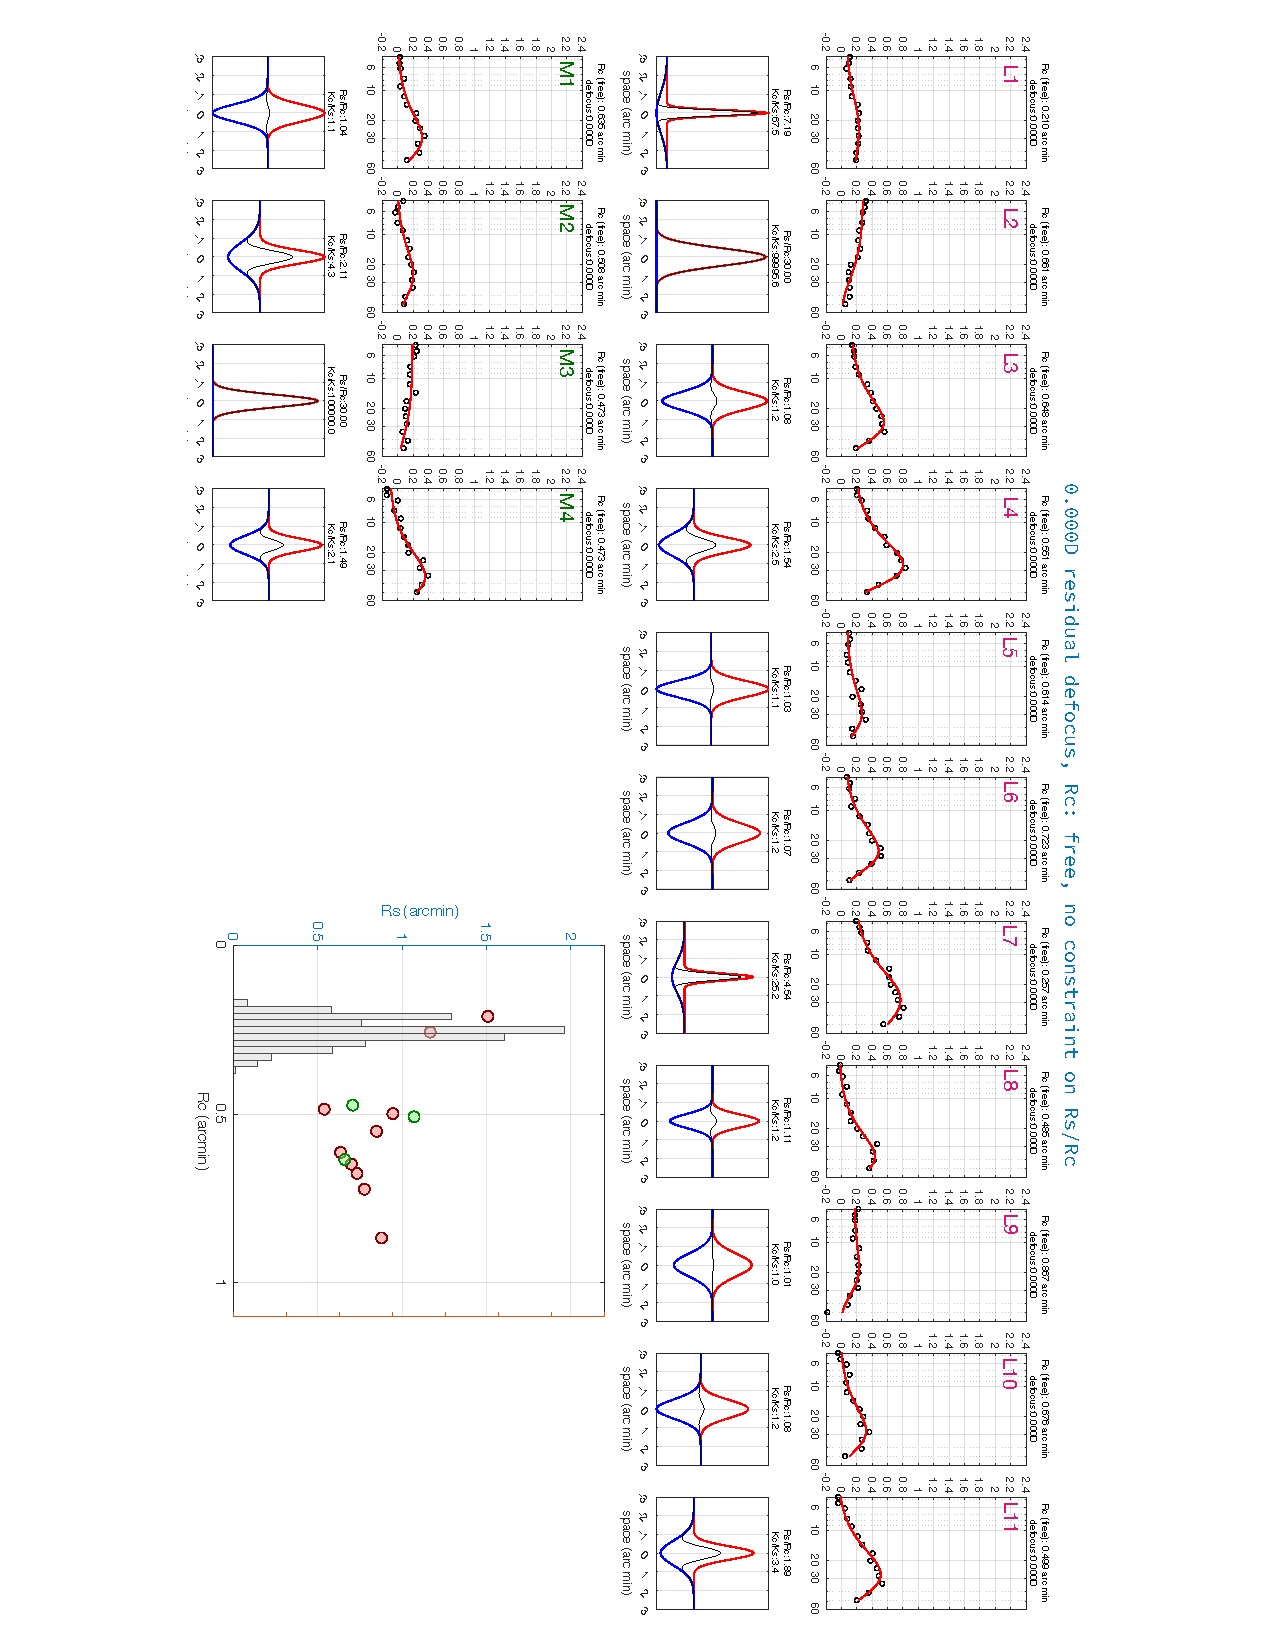
\includegraphics[width=7in]{Slide1.pdf} 
   \caption{Fitting the the raw spatial transfer function data using the free params DoG model}
   \label{fig:example}
\end{figure}

\begin{figure}[htbp] %  figure placement: here, top, bottom, or page
   \centering
   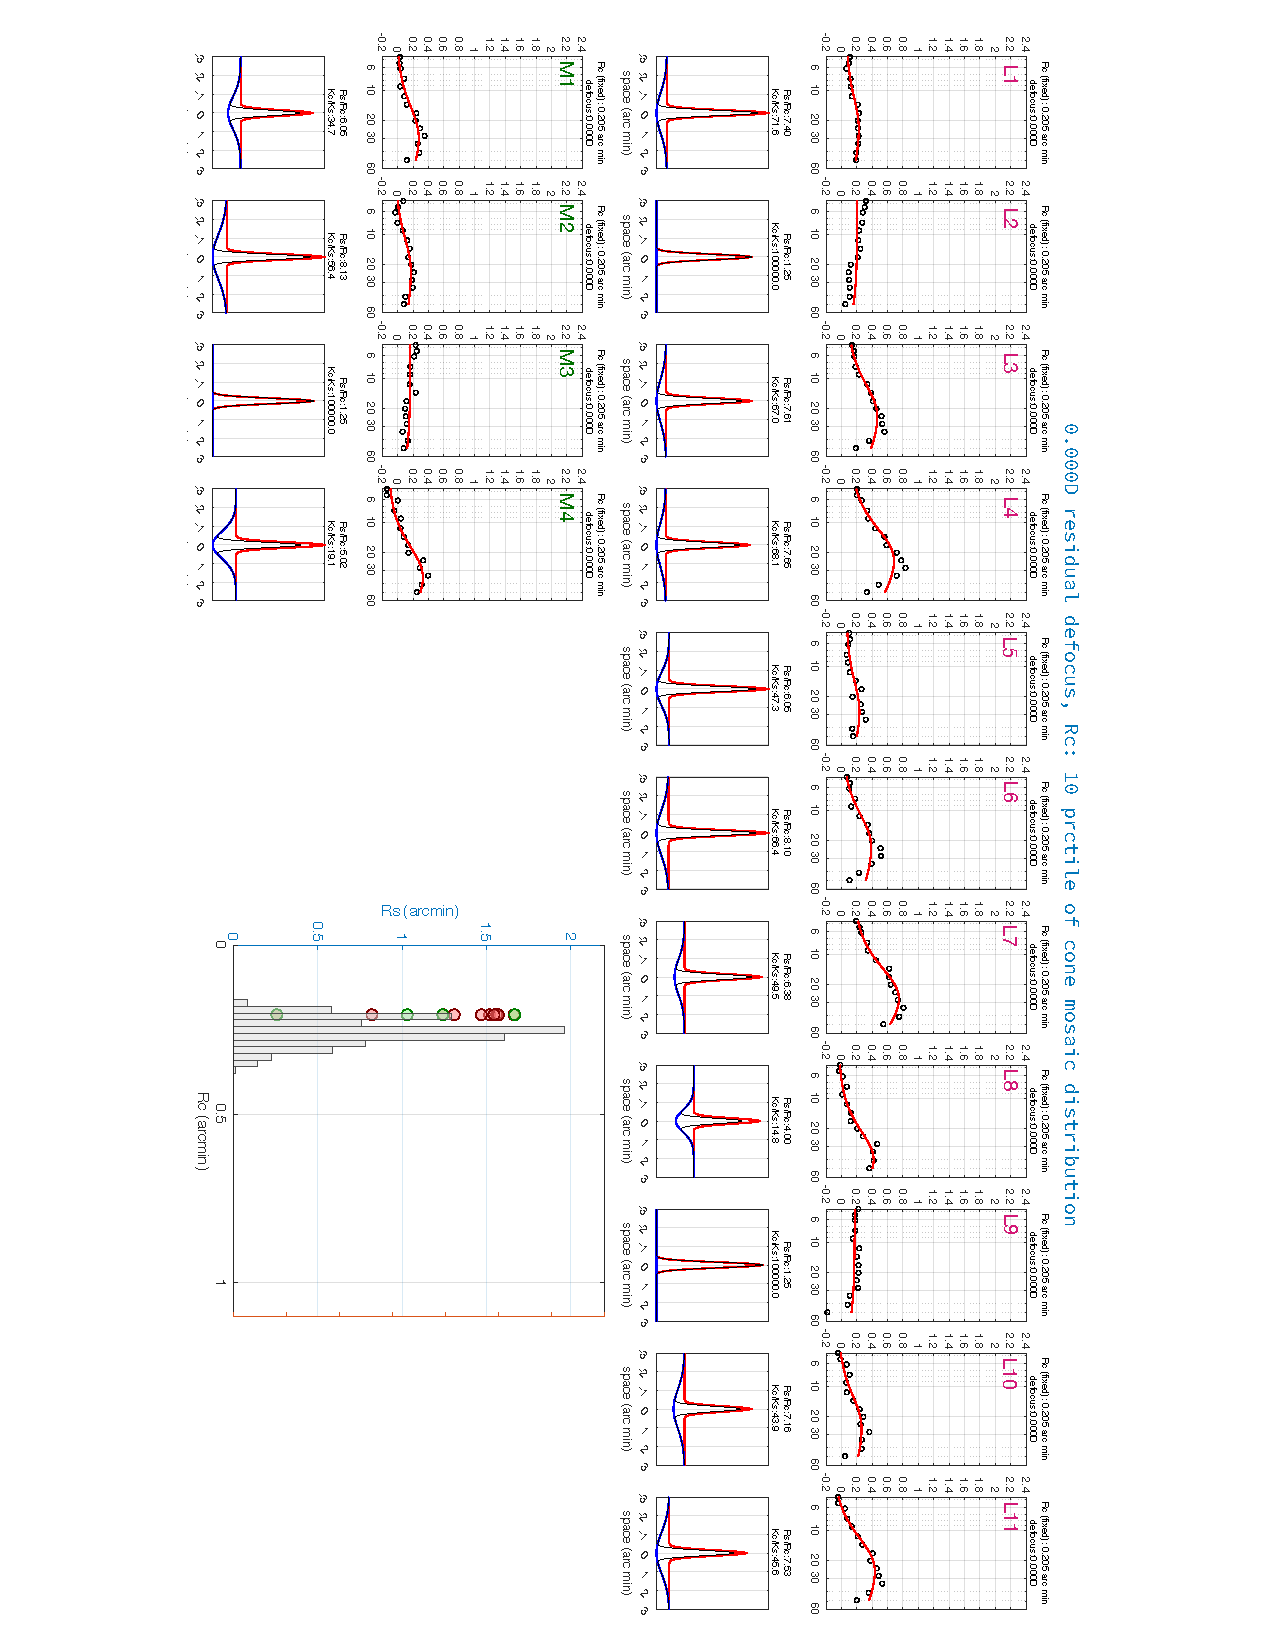
\includegraphics[width=7in]{Slide2.pdf} 
   \caption{Fitting the the raw spatial transfer function data using the Rc-fixed (10\%) DoG model}
   \label{fig:example}
\end{figure}

\begin{figure}[htbp] %  figure placement: here, top, bottom, or page
   \centering
   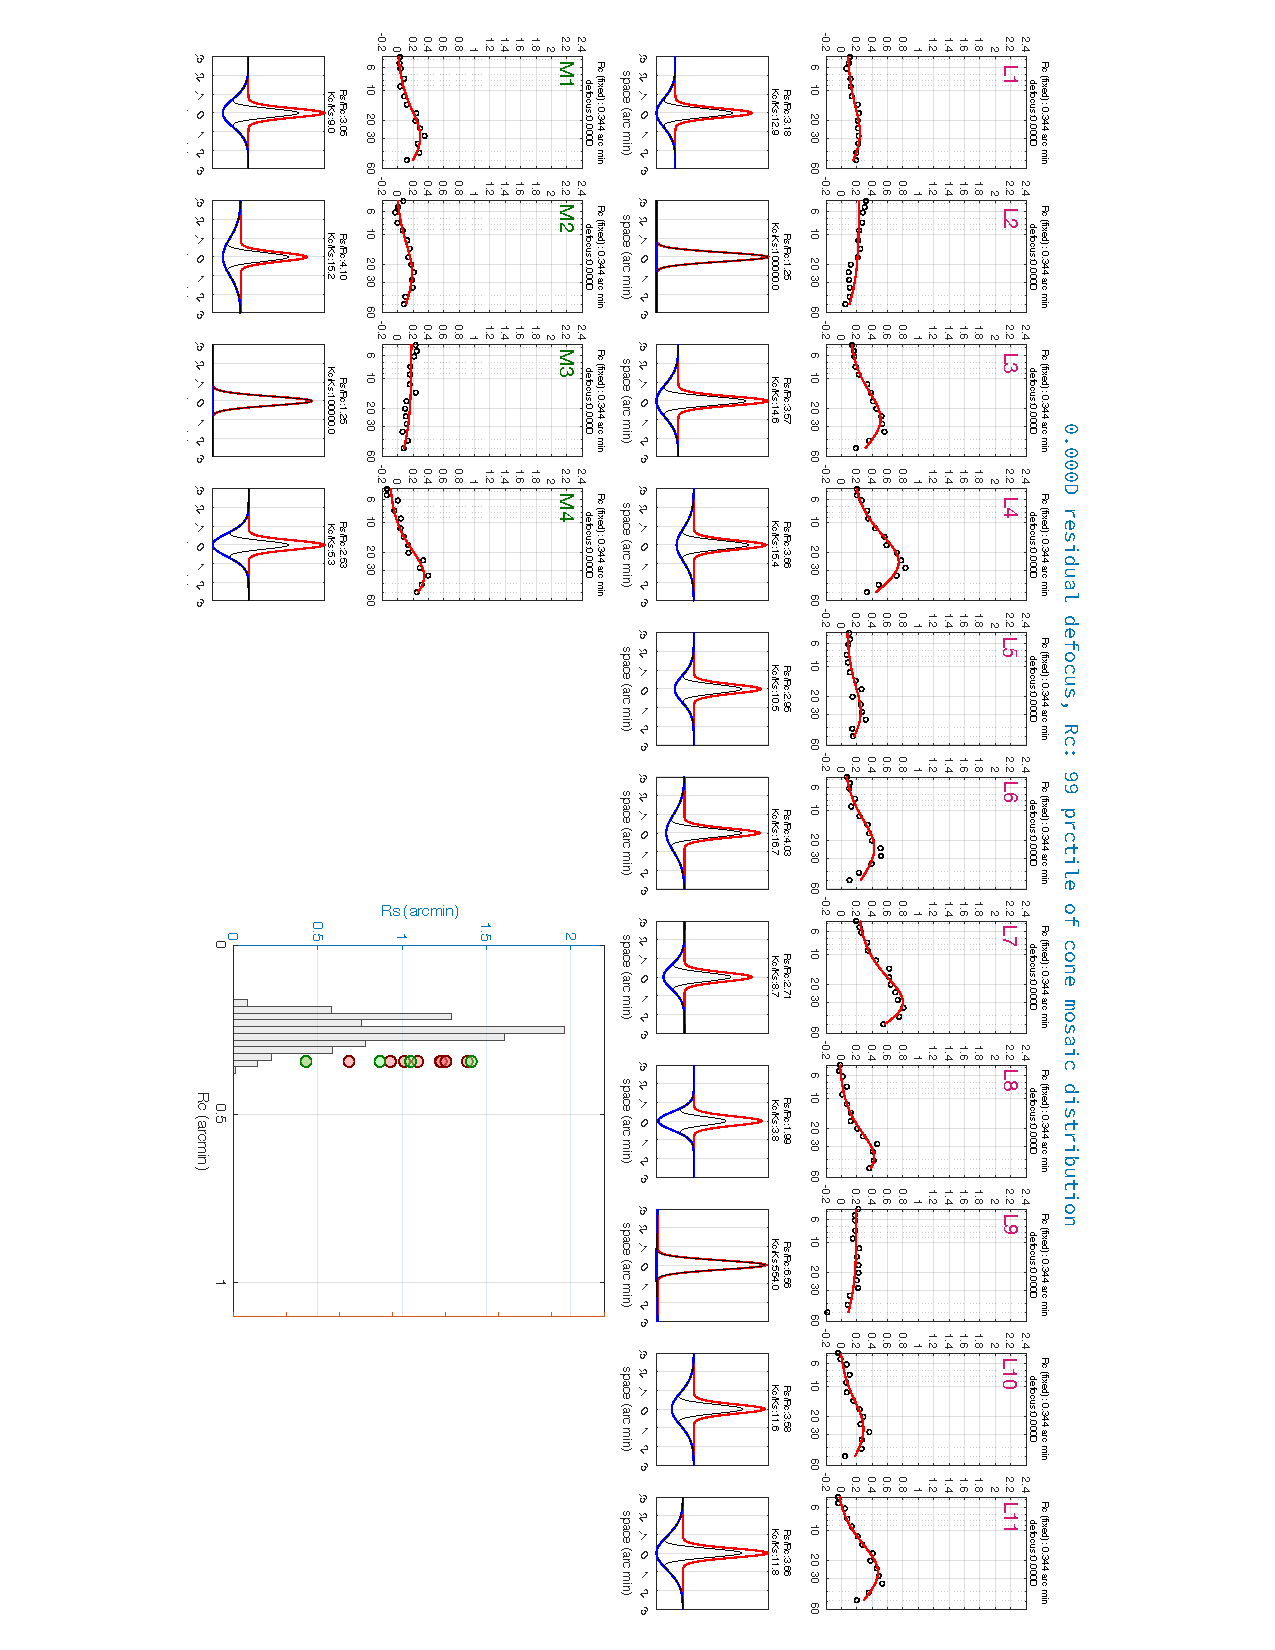
\includegraphics[width=7in]{Slide3.pdf} 
   \caption{Fitting the the raw spatial transfer function data using the Rc-fixed (99\%) DoG model}
   \label{fig:example}
\end{figure}

\begin{figure}[htbp] %  figure placement: here, top, bottom, or page
   \centering
   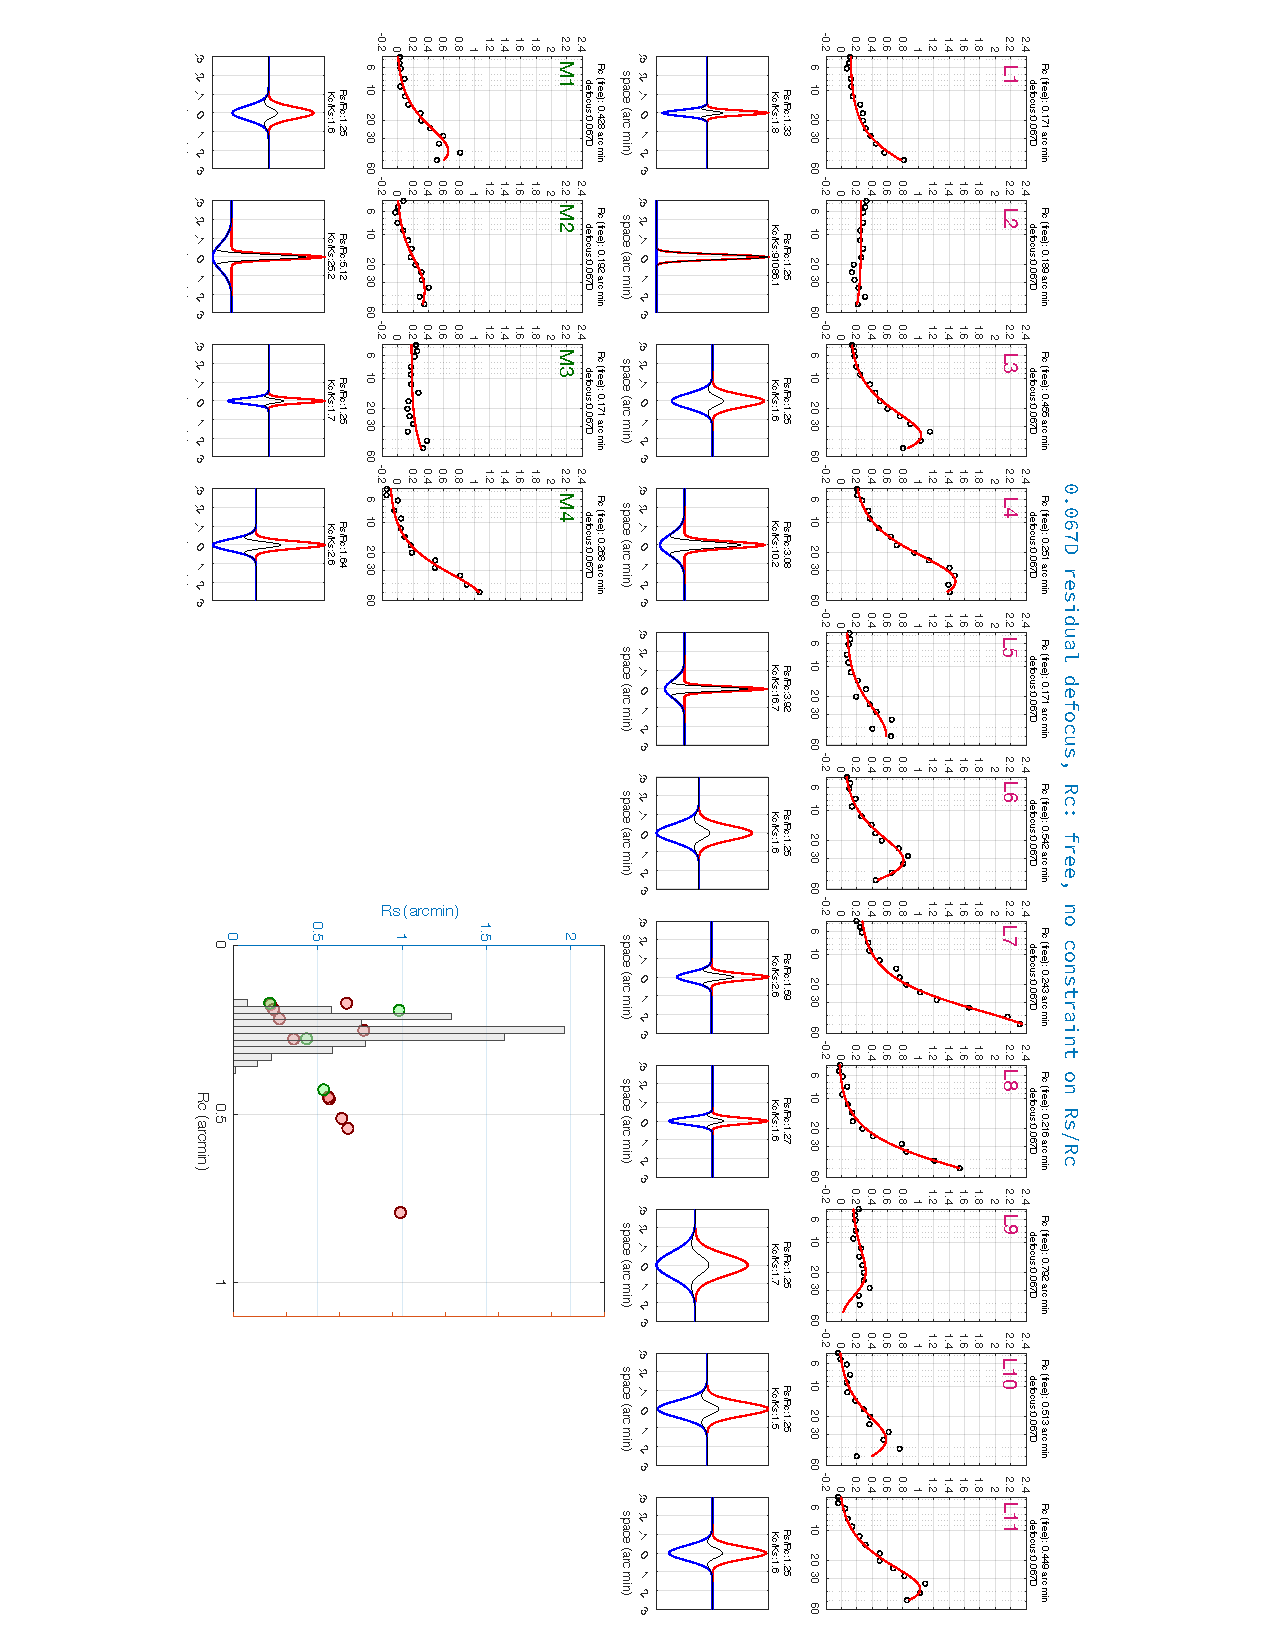
\includegraphics[width=7in]{Slide4.pdf} 
   \caption{Fitting the 0.067D deconvolved  data using the free params DoG model}
   \label{fig:example}
\end{figure}

\begin{figure}[htbp] %  figure placement: here, top, bottom, or page
   \centering
   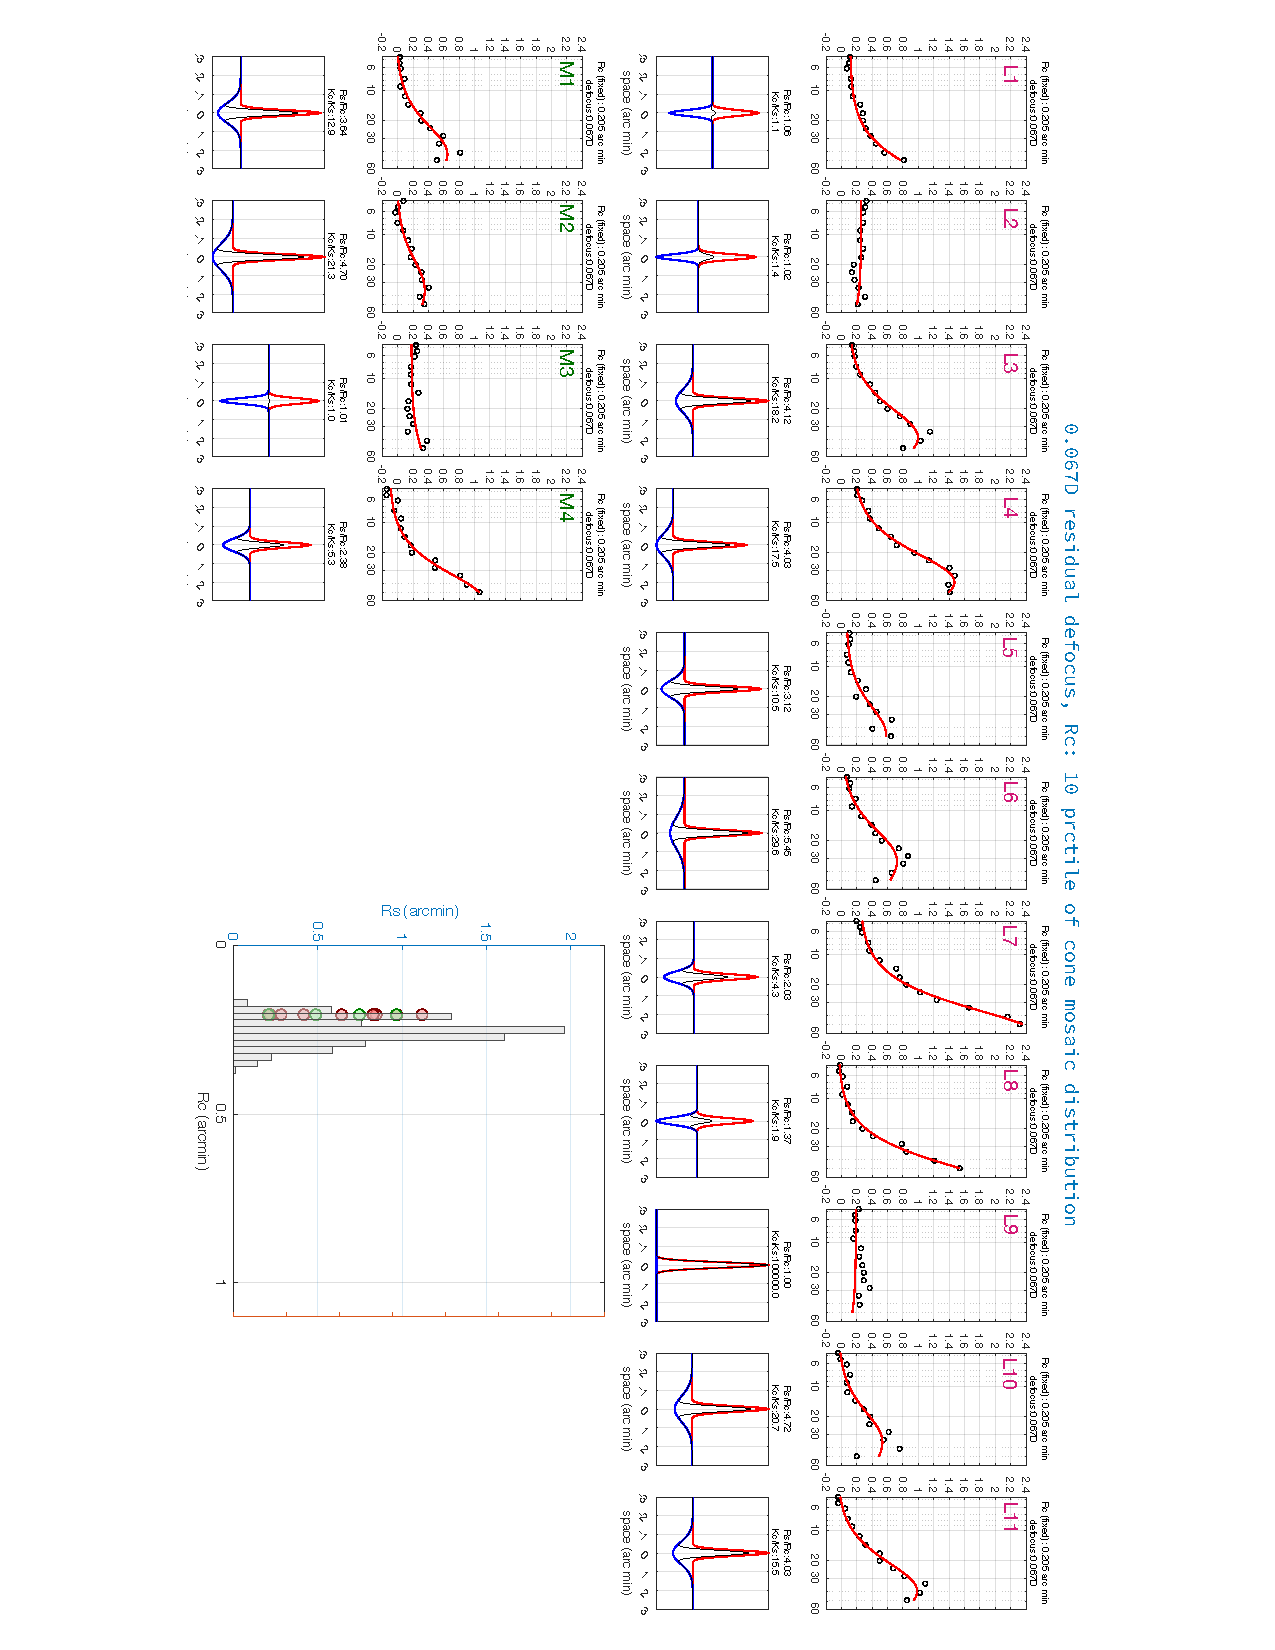
\includegraphics[width=7in]{Slide5.pdf} 
   \caption{Fitting the 0.067D deconvolved data using the Rc-fixed (10\%) DoG model}
   \label{fig:example}
\end{figure}

\begin{figure}[htbp] %  figure placement: here, top, bottom, or page
   \centering
   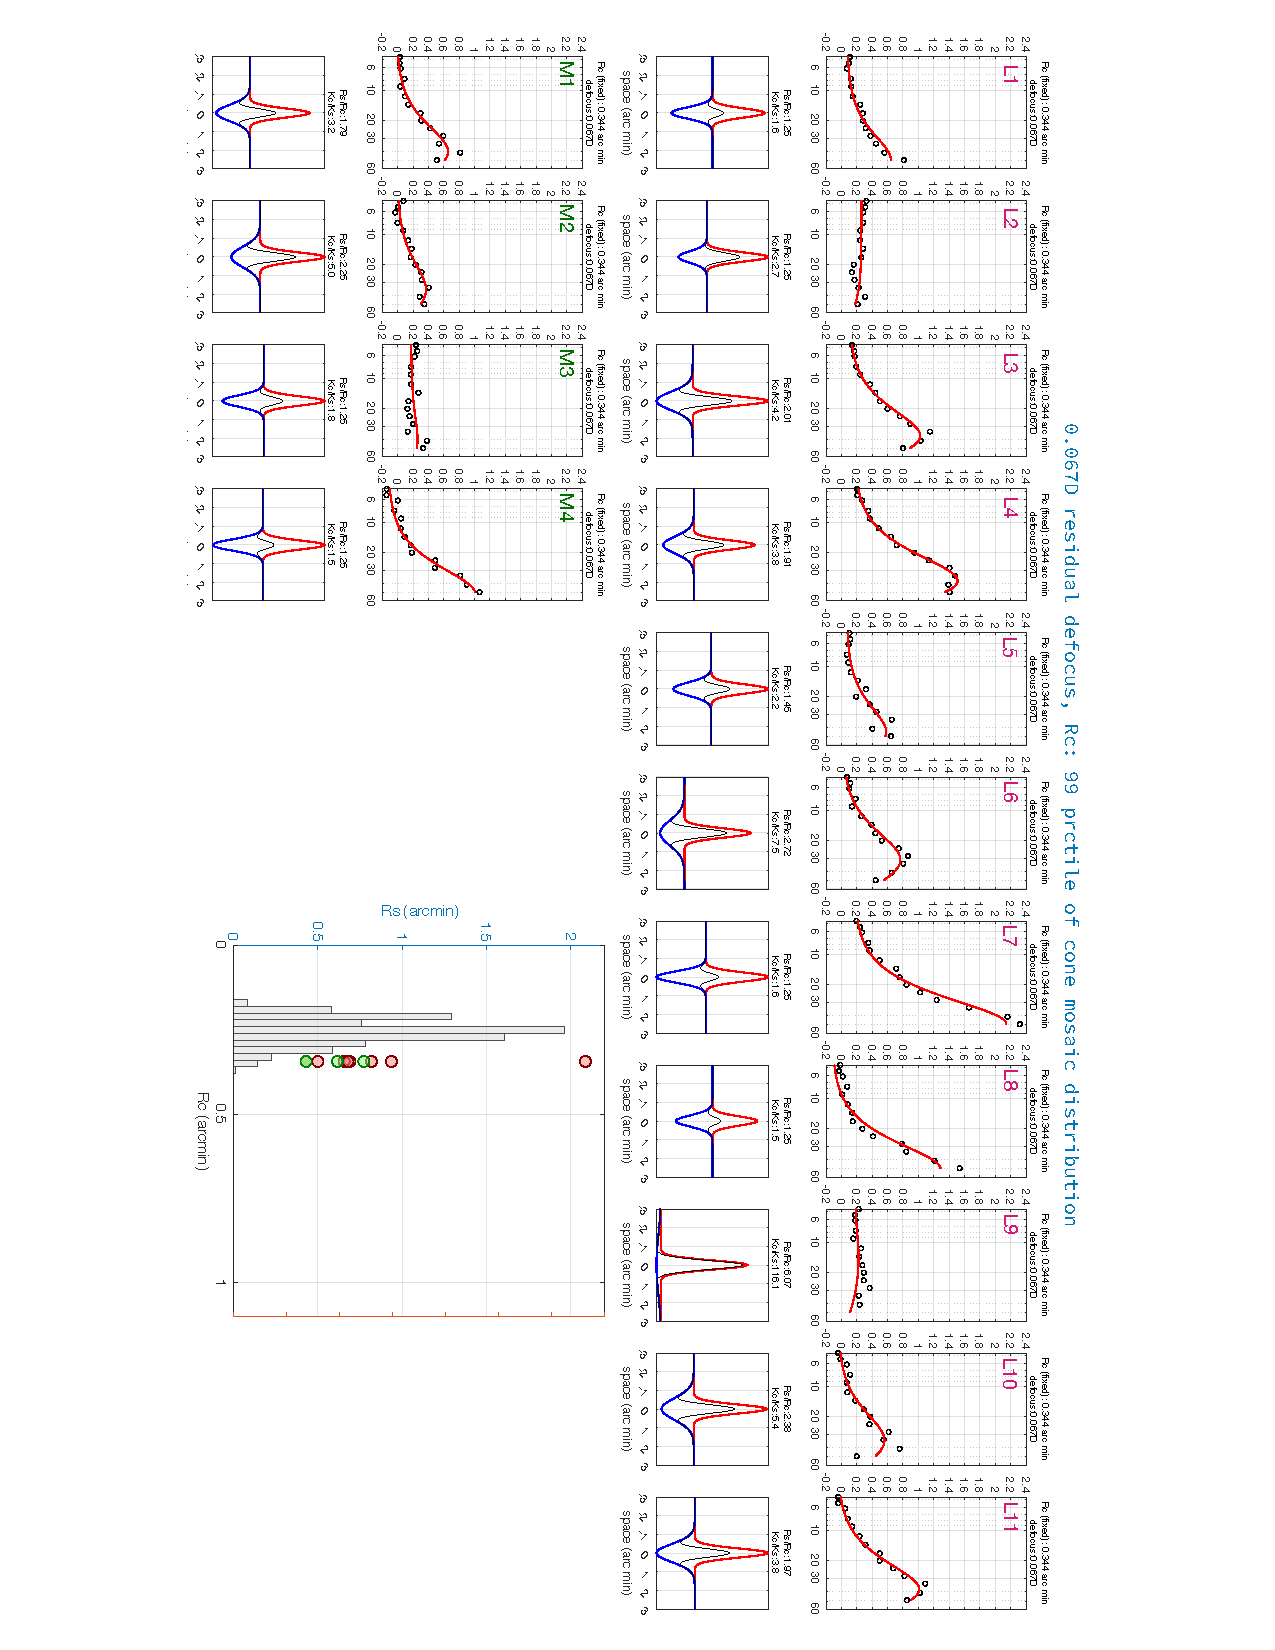
\includegraphics[width=7in]{Slide6.pdf} 
   \caption{Fitting the 0.067D deconvolved data using the Rc-fixed (99\%) DoG model}
   \label{fig:example}
\end{figure}

\begin{figure}[htbp] %  figure placement: here, top, bottom, or page
   \centering
   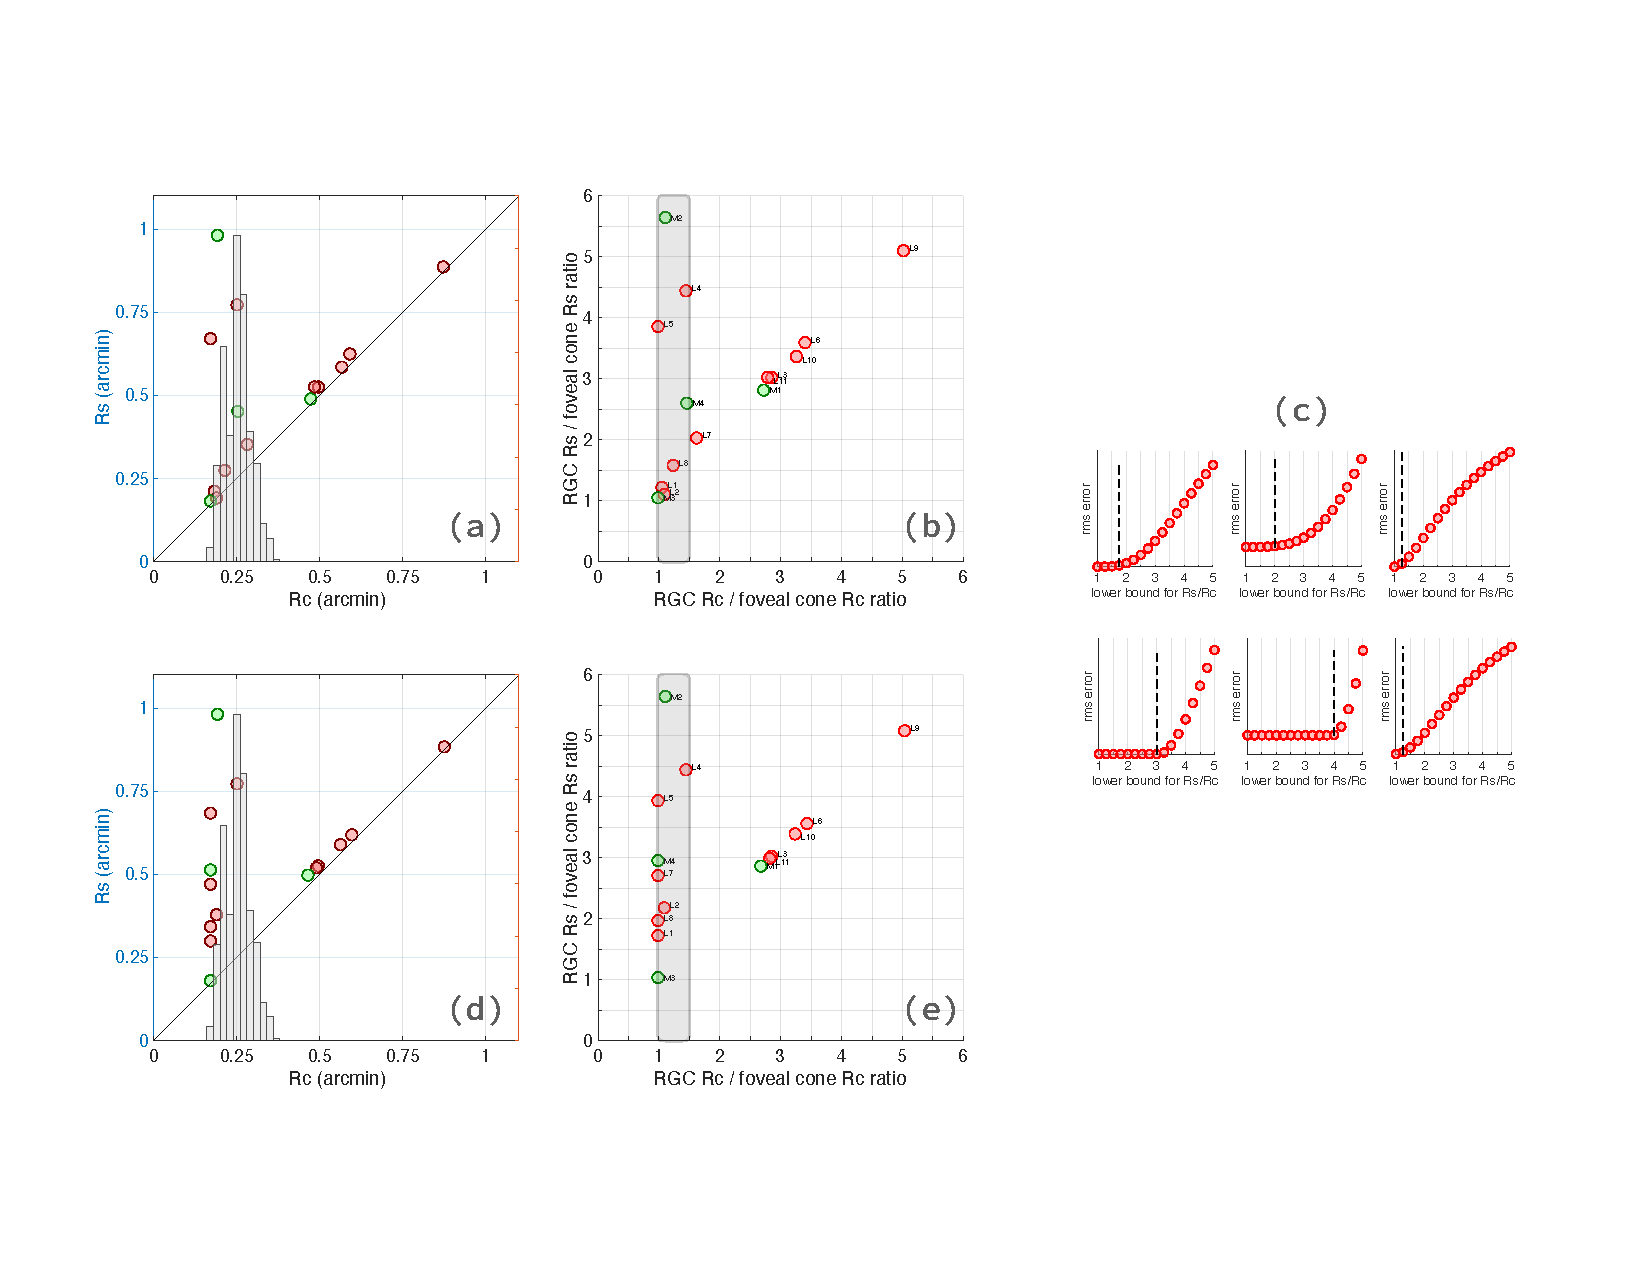
\includegraphics[width=8in]{Slide7.pdf} 
   \caption{Determining number of cone inputs to the RGC RF centers}
   \label{fig:example}
\end{figure}

\end{document}  